\documentclass[dvipsnames, svgnames,a4paper,11pt]{article}
\usepackage{todonotes}
% ----------------------------------------------------- 
%	加边框的命令
%	参考:https://tex.stackexchange.com/questions/531559/how-to-add-the-page-border-for-first-two-pages-in-latex
\usepackage{tikz}
\usetikzlibrary{calc}
\usepackage{eso-pic}
\AddToShipoutPictureBG{%
\begin{tikzpicture}[overlay,remember picture]
\draw[line width=0.6pt] % 边框粗细
    ($ (current page.north west) + (0.6cm,-0.6cm) $)
    rectangle
    ($ (current page.south east) + (-0.6cm,0.6cm) $); % 边框位置
\end{tikzpicture}}


\usepackage{xcolor}
\definecolor{c1}{HTML}{2752C9} % 目录颜色
\definecolor{c2}{RGB}{190,20,83} % 引用颜色

\usepackage{ctex}
\usepackage[top=28mm,bottom=28mm,left=15mm,right=15mm]{geometry} % 调整边距
\usepackage{hyperref} 
\hypersetup{
	colorlinks,
	linktoc = section, % 给目录加的超链接位置,选项有 section, page, all
	linkcolor = c1, % linkcolor 目录颜色
	citecolor = c1  % citecolor 引用颜色
}
\usepackage{amsmath,enumerate,multirow,float}
\usepackage{tabularx}
\usepackage{tabu}
\usepackage{subfig}
\usepackage{fancyhdr}
\usepackage{graphicx}
\usepackage{wrapfig}  
\usepackage{physics}
\usepackage{appendix}
\usepackage{amsfonts}
\usepackage{annotate-equations} % 公式标注
\usepackage{pgfplots} % pgf 绘图


% ---------------------------------------------------------------------
%	定义了两类colorbox
\usepackage{tcolorbox}
\tcbuselibrary{skins,breakable}
\newtcolorbox{tbox}[2][]{
    colframe=black!70!,
    breakable,
    enhanced,
    boxrule =0.5pt,
    title = {#2},
    fonttitle = \large\bfseries,
    drop fuzzy shadow,
    #1
}
\newtcolorbox[auto counter,number within=section]{question}[1][]{
  top=2pt,bottom=2pt,arc=1mm,
  boxrule=0.5pt,
  breakable,
  enhanced, % 跨页后不会显示下边框
  coltitle=c1!80!gray,
  colframe=c1,
  colback=c1!3!white,
  drop fuzzy shadow,
  title={思考题~\thetcbcounter:\quad},
  fonttitle=\bfseries,
  attach title to upper,
  #1
}

% ---------------------------------------------------------------------
%	利用 cleveref 改变引用格式,\cref 是引用命令
\usepackage{cleveref}
\crefformat{figure}{#2{\textcolor{c2}{图 #1}}#3} % 图片的引用格式
\crefformat{equation}{#2{(\textcolor{c2}{#1})}#3} % 公式的引用格式
\crefformat{table}{#2{\textcolor{c2}{表 #1}}#3} % 表格的引用格式


% ---------------------------------------------------------------------
%	页眉页脚设置
\fancypagestyle{plain}{\pagestyle{fancy}}
\pagestyle{fancy}
\lhead{\kaishu 中山大学物理与天文学院近代物理实验\uppercase\expandafter{\romannumeral1}} % 左边页眉,学院 + 课程
\rhead{\kaishu 材料真空兼容测试和等离子特性研究 实验报告} % 右边页眉,实验报告标题
\cfoot{\thepage} % 页脚,中间添加页码
\setlength{\headheight}{13.6pt}

% ---------------------------------------------------------------------
%	对目录、章节标题的设置
\renewcommand{\contentsname}{\centerline{\huge 目录}}
\usepackage{titlesec}
\usepackage{titletoc}
% \titleformat{章节}[形状]{格式}{标题序号}{序号与标题间距}{标题前命令}[标题后命令]
\titleformat{\section}{\centering\LARGE}{}{1em}{}
\newcommand{\nsection}[3]{%
    \section{#1 #2 \hspace{11pt} \textbf{#3}}%
}

% ---------------------------------------------------------------------
%   listing代码环境设置
\usepackage{listings}
\lstloadlanguages{python}
\lstdefinestyle{pythonstyle}{
backgroundcolor=\color{gray!5},
language=python,
frameround=tftt,
frame=shadowbox, 
keepspaces=true,
breaklines,
columns=spaceflexible,                   
basicstyle=\ttfamily\small, % 基本文本设置,字体为 teletype,大小为 small
keywordstyle=[1]\color{c1}\bfseries, 
keywordstyle=[2]\color{Red!70!black},   
stringstyle=\color{Purple},       
showstringspaces=false,
commentstyle=\ttfamily\scriptsize\color{green!40!black}, % 注释文本设置,字体为 teletype,大小为 scriptsize
tabsize=2,
morekeywords={as},
morekeywords=[2]{np, plt, sp},
numbers=left, % 代码行数,位置在左
numberstyle=\it\tiny\color{gray}, % 代码行数的数字字体设置
stepnumber=1,
rulesepcolor=\color{gray!30!white}
}


% ---------------------------------------------------------------------
%	将表格封装起来
\newcommand{\scoresTable}[8]{
    \begin{table}
        \renewcommand\arraystretch{1.7}
        \begin{tabularx}{\textwidth}{
                |X|X|X|X
                |X|X|X|X|}
            \hline
            \multicolumn{2}{|c|}{预习报告} & \multicolumn{2}{|c|}{实验记录} & \multicolumn{2}{|c|}{分析讨论} & \multicolumn{2}{|c|}{总成绩} \\
            \hline
            \centering#1&\centering#2 &\centering#3 &\centering#4 &\centering#5 &\centering#6 &\centering#7 &{\centering#8} \\
            \hline
        \end{tabularx}
    \end{table}
}
\newcommand{\infoTable}[6]{
    \begin{table}
        \renewcommand\arraystretch{1.7}
        \begin{tabularx}{\textwidth}{|X|X|X|X|}
        \hline
        专业:& #1 &年级:& #2\\
        \hline
        姓名:& #3   & 学号:&#4\\
        \hline
        实验时间:&#5 & 教师签名:&#6 \\
        \hline
        \end{tabularx}
    \end{table}
}

% ---------------------------------------------------------------------
%	其他设置
\def\degree{${}^{\circ}$} % 角度
\graphicspath{{./images/}} % 插入图片的相对路径
\allowdisplaybreaks[4]  %允许公式跨页

\usetikzlibrary{patterns,decorations.markings,arrows.meta,bending} % TikZ 包的拓展 % 导入模板的相关设置
\usepackage{lipsum}
\usepackage{amsmath}
\usepackage{array}

\usepackage{tabularx}
\usepackage{graphicx}


\begin{document}

\scoresTable{}{}{}{}{}{}{}{}

% \infoTable{专业}{年级}{姓名}{学号}{实验时间}{教师签名}
\infoTable{物理学}{2022级}{丁侯凯}{22344009}{}{}

\begin{center}
	\LARGE D1 \quad 实验名称
\end{center}

\textbf{【实验报告注意事项】}
\begin{enumerate}
	\item 实验报告由三部分组成:
	\begin{enumerate}
		\item 预习报告:(提前一周)认真研读\underline{\textbf{实验讲义}},弄清实验原理;实验所需的仪器设备、用具及其使用(强烈建议到实验室预习),完成课前预习思考题;了解实验需要测量的物理量,并根据要求提前准备实验记录表格(第一循环实验已由教师提供模板,可以打印)。预习成绩低于10分(共20分)者不能做实验。
	    \item 实验记录:认真、客观记录实验条件、实验过程中的现象以及数据。实验记录请用珠笔或者钢笔书写并签名(\textcolor{red}{\textbf{用铅笔记录的被认为无效}})。\textcolor{red}{\textbf{保持原始记录,包括写错删除部分,如因误记需要修改记录,必须按规范修改。}}(不得输入电脑打印,但可扫描手记后打印扫描件);离开前请实验教师检查记录并签名。
	    \item 分析讨论:处理实验原始数据(学习仪器使用类型的实验除外),对数据的可靠性和合理性进行分析;按规范呈现数据和结果(图、表),包括数据、图表按顺序编号及其引用;分析物理现象(含回答实验思考题,写出问题思考过程,必要时按规范引用数据);最后得出结论。
	\end{enumerate}
	\textbf{实验报告就是将预习报告、实验记录、和数据处理与分析合起来,加上本页封面。}
	\item 每次完成实验后的一周内交\textbf{实验报告}(特殊情况不能超过两周)。
	\item 除实验记录外,实验报告其他部分建议双面打印。
\end{enumerate}


\clearpage
\tableofcontents
\clearpage

\setcounter{section}{0}
\nsection{XX}{实验名称}{预习报告}
	
\subsection{实验目的}
\begin{enumerate}
	\item 了解……
\end{enumerate}

\subsection{仪器用具}
\begin{table}[htbp]
	\centering
	\renewcommand\arraystretch{1.6}
	% \setlength{\tabcolsep}{10mm}
	\begin{tabular}{p{0.05\textwidth}|p{0.20\textwidth}|p{0.05\textwidth}|p{0.5\textwidth}}
	\hline
	编号& 仪器用具名称 & 数量 &  主要参数(型号,测量范围,测量精度等) \\
	\hline
	1& &1 & \\
	2& &1 & \\
	3& &1 &  \\
	

	\hline
\end{tabular}
\end{table}

\subsection{原理概述}
		\subsubsection{XXX原理}


		\subsubsection{工作原理}
			
		\subsubsection{公式推导}

		

\subsection{实验安全注意事项}
\begin{enumerate}
	\item ……
\end{enumerate}

\clearpage
\subsection{现场预习报告思考题}
	\begin{question}
		请写出问题
	\end{question}
	在这里回答

		%插入图片的事例
	% \begin{figure}[htbp]
	% 	\centering
	% 	\includegraphics[width=0.75\textwidth]{XX图.jpg}
	% 	\caption{XX图}
	% 	\label{fig:XX}
	% \end{figure}
		%插入公式事例
	% \begin{equation}
	% v(t) = s(t) +n(t)
	% \label{eq:1}
	% \end{equation}
	
		%插入多行对齐公式事例
	% \begin{align}
	% 	u_{px}(t) &= u_r(t)u_a(t) \nonumber \\
	% 			  &= A_I[s(t)\sin(\omega_m t + \theta)\sin(\omega_r t) + n(t)\sin(\omega_r t)] \nonumber \\
	% 			  &= A_I { \frac{s(t)}{2} \left[ \cos((\omega_m - \omega_r)t + \theta) - \cos((\omega_m + \omega_r)t + \theta) \right] + n(t)\sin(\omega_r t) } \label{eq:2}
	% \end{align}

%  给出段落间的空行  \vspace{1cm}

	%插入表格事例
% \begin{table}[ht]
	% \centering
	% \begin{tabularx}{\textwidth}{|c|X|X|X|}
	% 	\hline
	% 	% 第一行表头
	% 	时间常数 & R波形  & X波形  & Y波形 \\
	% 	\hline
	% 	% 数据行 1
	% 	10us & 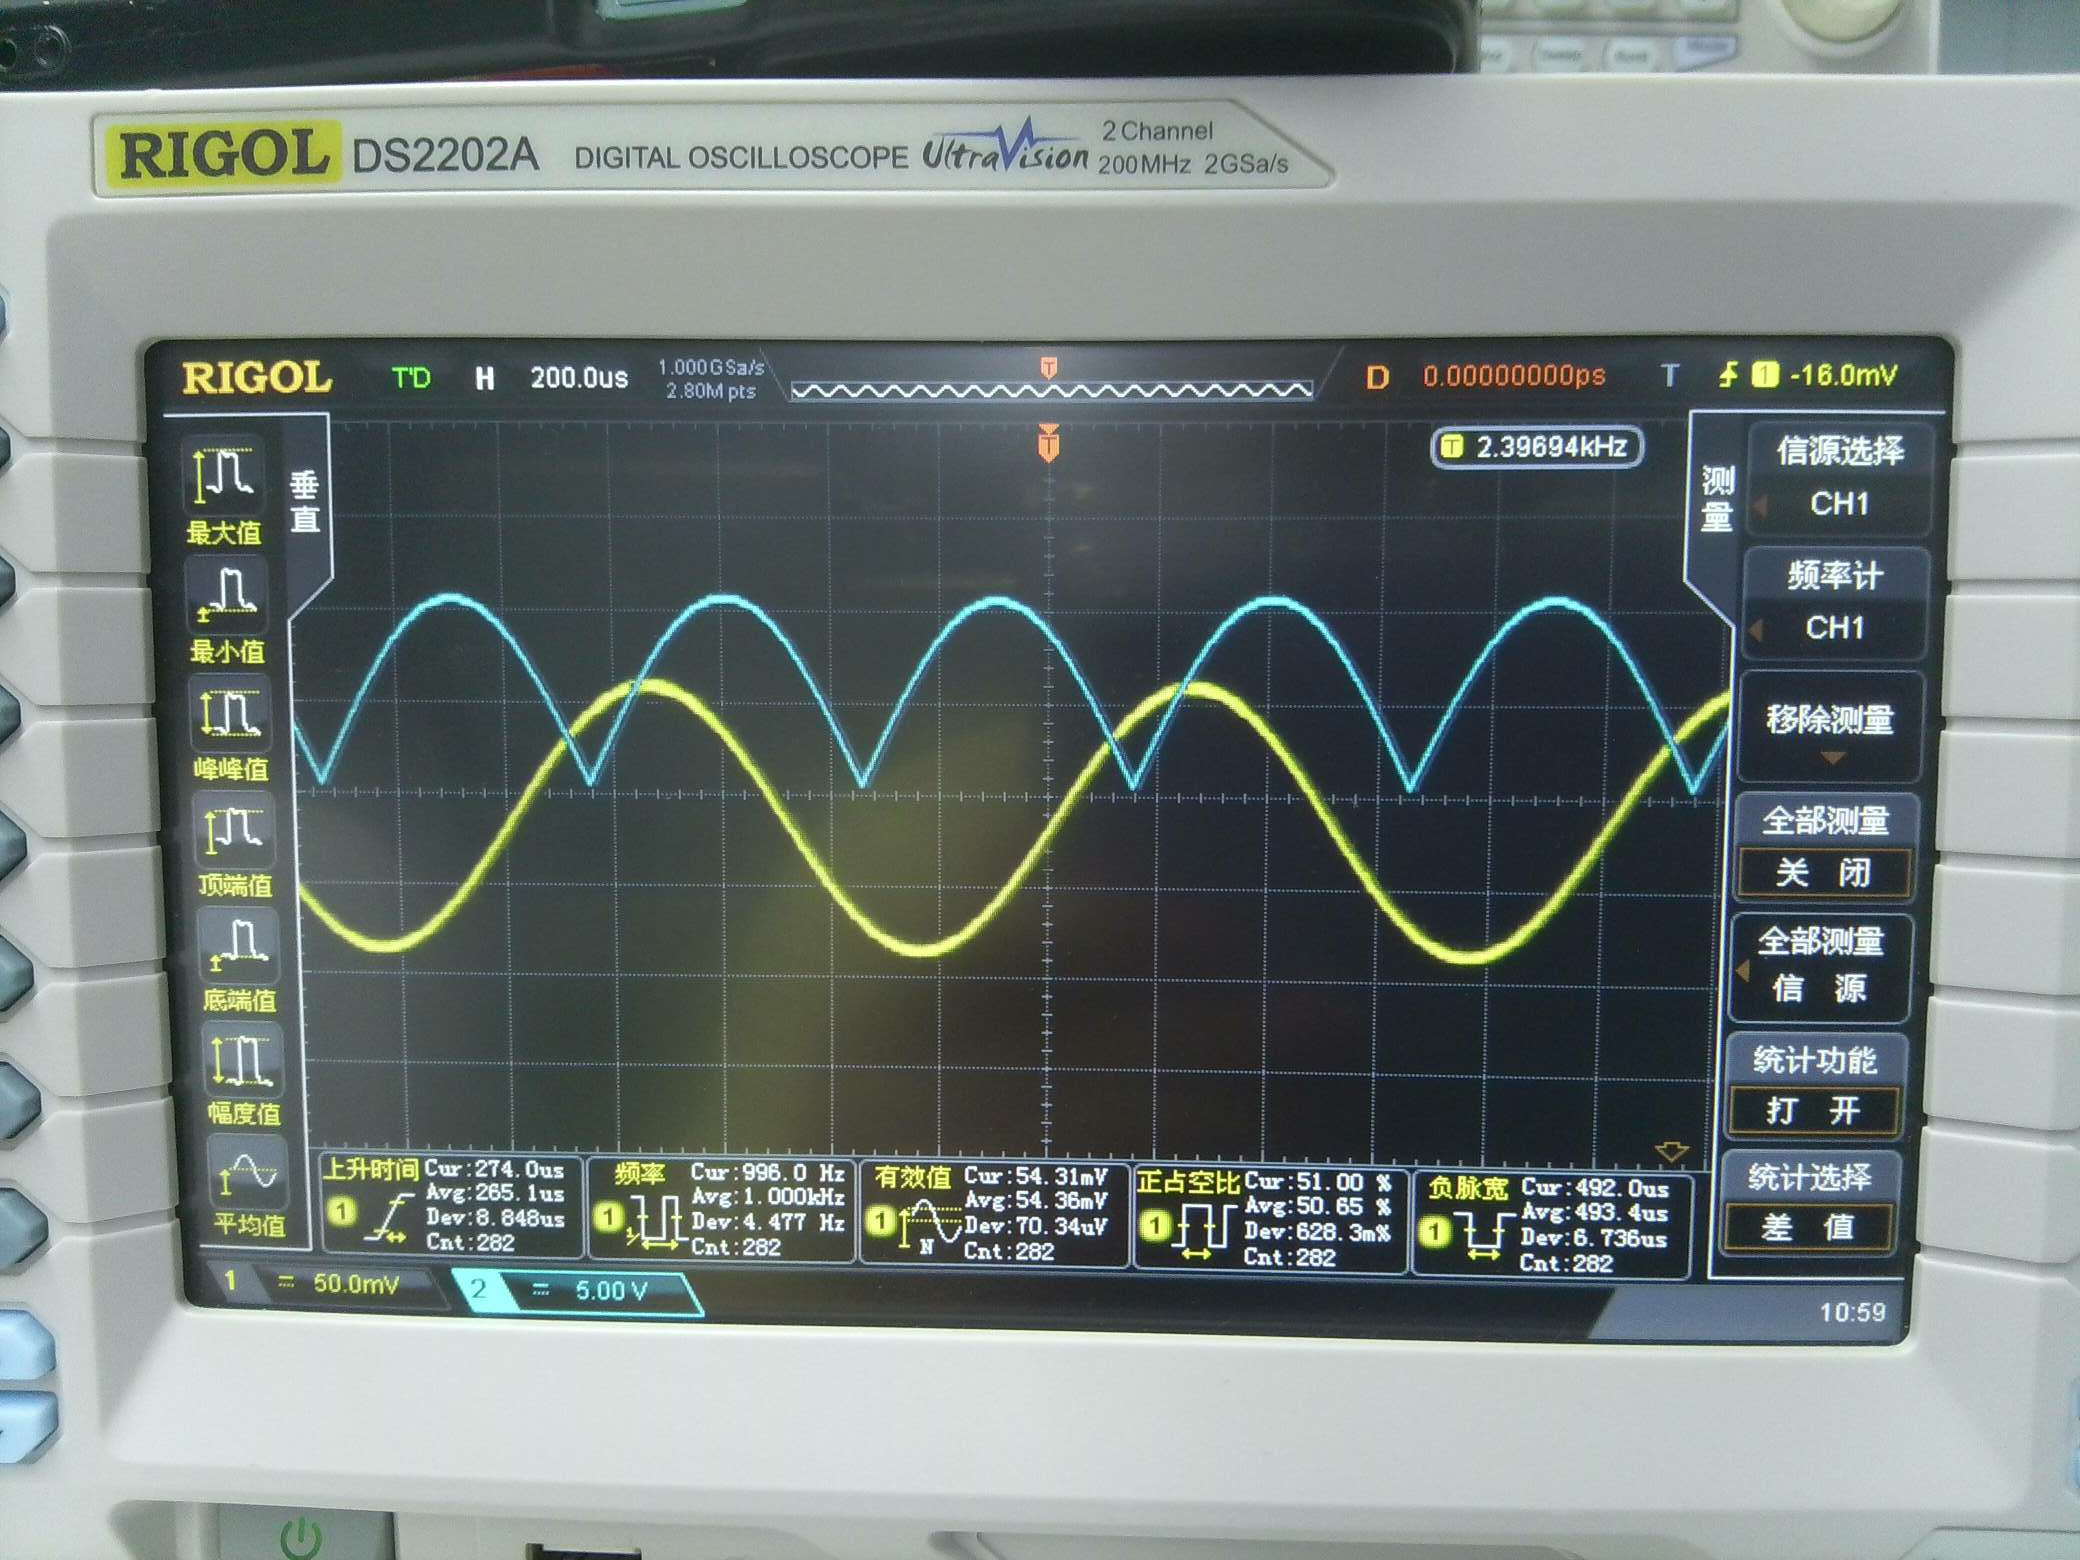
\includegraphics[width=3cm]{示波器图片1.1.png} & \includegraphics[width=3cm]{1.2.png}&\includegraphics[width=3cm]{1.3.png} \\
	% 	\hline
	% 	% 数据行 2
	% 	100us &\includegraphics[width=3cm]{2.1.png} & \includegraphics[width=3cm]{2.2.png} & \includegraphics[width=3cm]{2.3.png}\\
	% 	\hline
	% 	% 数据行 3
	% 	1ms &\includegraphics[width=3cm]{3.1.png} & \includegraphics[width=3cm]{3.2.png} & 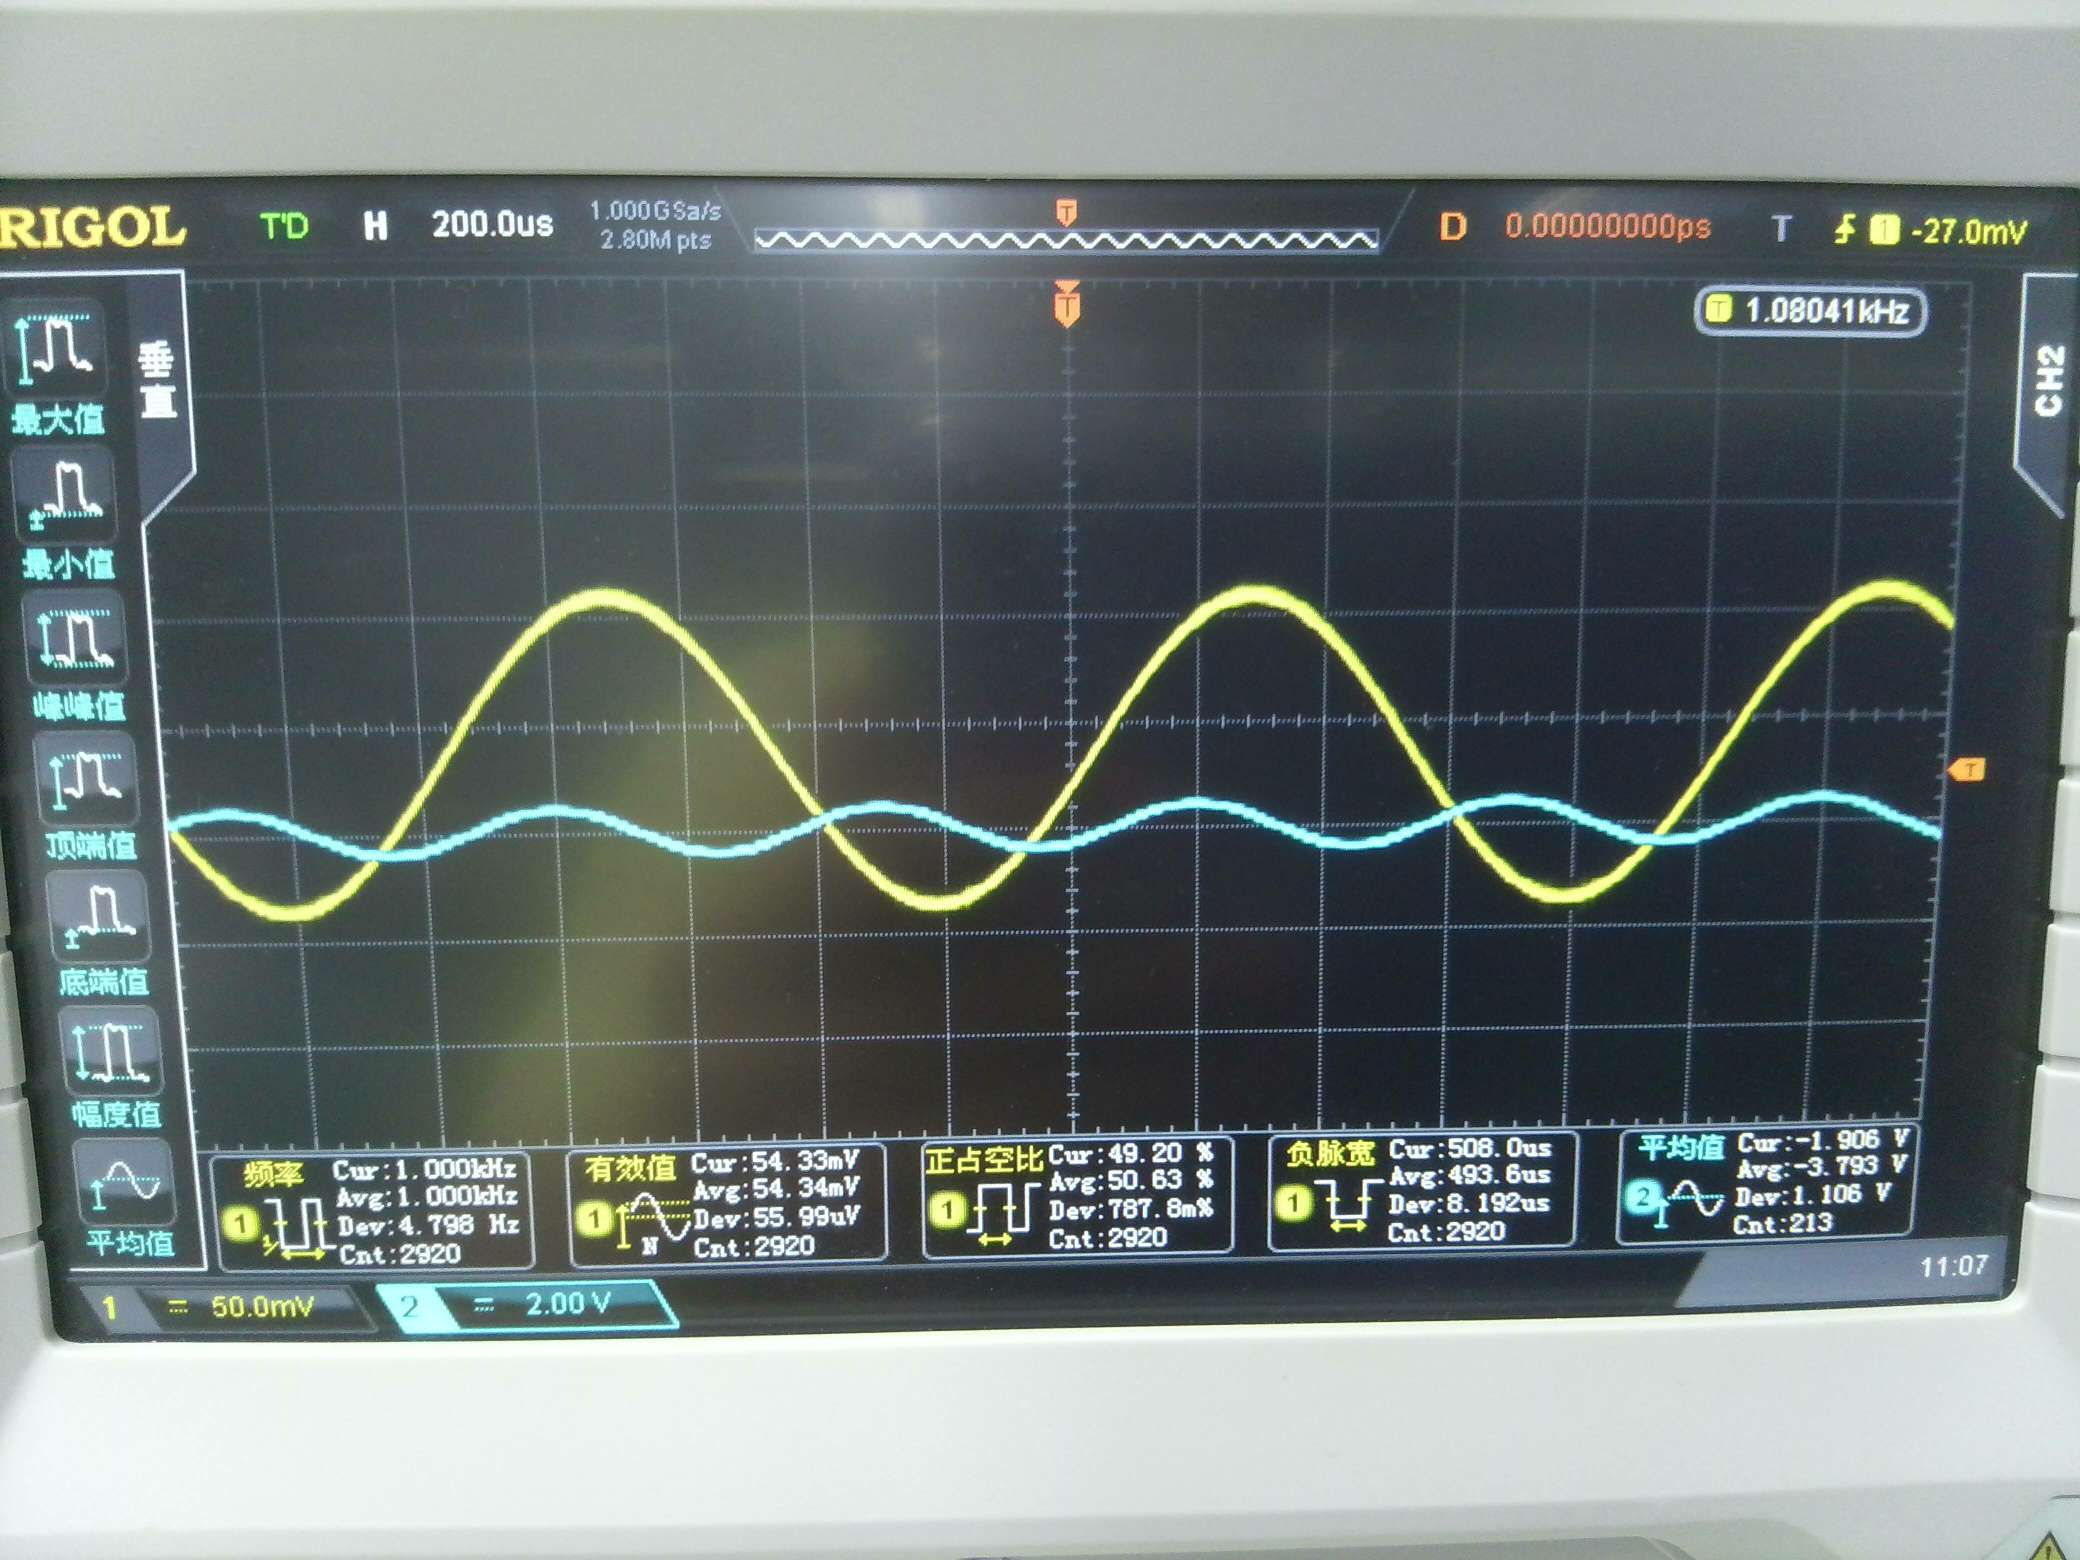
\includegraphics[width=3cm]{3.3.png} \\
	%   \hline
	% \end{tabularx}
	% \caption{陡降为6dB/oct时,改变时间常数,低通滤波器配合乘法器解调过程探究记录}
	% \label{tab:1}
% \end{table}

%多行并列图片
	% \begin{figure}[htbp]
	% 	\centering
	% 	% 第一张图片
	% 	\begin{subfigure}[b]{0.45\textwidth} % 子图的宽度设置为页面宽度的45%
	% 		\centering
	% 		\includegraphics[width=\textwidth]{image1.jpg}
	% 		\caption{第一张图}
	% 		\label{fig:image1}
	% 	\end{subfigure}
	% 	\hfill % 增加两张图片之间的间距
	% 	% 第二张图片
	% 	\begin{subfigure}[b]{0.45\textwidth}
	% 		\centering
	% 		\includegraphics[width=\textwidth]{image2.jpg}
	% 		\caption{第二张图}
	% 		\label{fig:image2}
	% 	\end{subfigure}
	% 	\caption{并排显示的两张图片示例}
	% 	\label{fig:two_images}
	% \end{figure}




\clearpage
\begin{table}
	\renewcommand\arraystretch{1.7}
	\centering
	\begin{tabularx}{\textwidth}{|X|X|X|X|}
	\hline
	专业:& 物理学 &年级:& 2019级 \\
	\hline
	姓名: & 丁侯凯& 学号:&22344009\\
	\hline
	室温:& & 实验地点: & \\
	\hline
	学生签名:& 
\includegraphics[width=2cm]{签名.jpg}      & 评分: &\\
	\hline
	实验时间:& & 教师签名:&\\
	\hline
	\end{tabularx}
\end{table}

\nsection{XX}{XX实验}{实验记录}
\subsection{实验内容和步骤}
	\subsubsection{实验步骤XX}
		\begin{enumerate}
		\item ……
		\end{enumerate}


	\subsubsection{XX的关系}
		\begin{enumerate}
		\item ……
		\end{enumerate}

		
\clearpage
\begin{table}
	\renewcommand\arraystretch{1.7}
	\begin{tabularx}{\textwidth}{|X|X|X|X|}
	\hline
	专业:& 物理学 &年级:& 2022级\\
	\hline
	姓名: &丁侯凯 & 学号:&22344009 \\
	\hline
    日期:& & 评分: &\\
	\hline
	\end{tabularx}
\end{table}

\nsection{XX}{XX实验}{分析与讨论}
\subsection{实验数据分析}

	\textbf{【问题一】XX?}

	


\subsection{实验报告思考题}
	\begin{question}
		请给出问题
	\end{question}
		请写出答案

		

\clearpage
% ---------------------------------------------------------------------
%   参考文献
%   注:使用参考文献时应按照xelatex->bibtex->xelatex->xelatex顺序进行编译
\phantomsection
\addcontentsline{toc}{section}{参考文献}
\bibliographystyle{unsrt} % 调整参考文献的格式,可供选择的有 plain, unsrt, alpha, abbrv, ieeetr, acm, siam, apalike 等。
\bibliography{myref}

% \clearpage
% \appendix
% \appendixpage
% \addappheadtotoc

% \begin{tbox}{字体设置(中文)}
% \begin{enumerate}
% 	\item 宋体:{\songti 山有扶苏,隰有荷华}
% 	\item 仿宋:{\fangsong 山有扶苏,隰有荷华}
% 	\item 黑体:{\heiti 山有扶苏,隰有荷华}
% 	\item 楷书:{\kaishu 山有扶苏,隰有荷华}
% \end{enumerate}
% \end{tbox}

% \begin{tbox}{Set font(English)}
% \begin{enumerate}
% 	\item roman:\quad{\rmfamily Hello world!}
% 	\item sans-serif:\quad{\sffamily Hello world!}
% 	\item typewriter:\quad{\ttfamily Hello world!}
% \end{enumerate}
% \end{tbox}

% \begin{tbox}{公式}
% 	无编号公式
%     \begin{equation*}
%         J(\theta) = \mathbb{E}_{\pi_\theta}[G_t] = \sum_{s\in\mathcal{S}} d^\pi (s)V^\pi(s)=\sum_{s\in\mathcal{S}} d^\pi(s)\sum_{a\in\mathcal{A}}\pi_\theta(a|s)Q^\pi(s,a)
%     \end{equation*}
% $$ J(\theta) = \mathbb{E}_{\pi_\theta}[G_t] = \sum_{s\in\mathcal{S}} d^\pi (s)V^\pi(s)=\sum_{s\in\mathcal{S}} d^\pi(s)\sum_{a\in\mathcal{A}}\pi_\theta(a|s)Q^\pi(s,a) $$
%     有编号公式
%     \begin{equation}
%         J(\theta) = \mathbb{E}_{\pi_\theta}[G_t] = \sum_{s\in\mathcal{S}} d^\pi (s)V^\pi(s)=\sum_{s\in\mathcal{S}} d^\pi(s)\sum_{a\in\mathcal{A}}\pi_\theta(a|s)Q^\pi(s,a)
%     \end{equation}
%     \begin{equation}
%         J(\theta) = \mathbb{E}_{\pi_\theta}[G_t] = \sum_{s\in\mathcal{S}} d^\pi (s)V^\pi(s)=\sum_{s\in\mathcal{S}} d^\pi(s)\sum_{a\in\mathcal{A}}\pi_\theta(a|s)Q^\pi(s,a)
%     \end{equation}
% 	波尔文积分
%     \[
%     \begin{cases}
%         \vspace{0.2cm}
%         \displaystyle{\int_{0}^{\infty} \frac{\sin(x)}{x}\dd{x} = \frac{\pi}{2}}\\
%         \vspace{0.2cm}
%         \displaystyle{\int_{0}^{\infty} \frac{\sin(x)}{x} \frac{\sin(x/3)}{x/3}\dd{x} = \frac{\pi}{2}} \\
%         \vspace{0.2cm}\cdot\cdot\cdot\\
%         \vspace{0.2cm}
%         \displaystyle{\int_{0}^{\infty} \frac{\sin(x)}{x} \frac{\sin(x/3)}{x/3} \cdot\cdot\cdot \frac{\sin(x/13)}{x/13}\dd{x} = \frac{\pi}{2}}\\
%         \displaystyle{\int_{0}^{\infty} \frac{\sin(x)}{x} \frac{\sin(x/3)}{x/3} \cdot\cdot\cdot \frac{\sin(x/15)}{x/15}\dd{x} = \frac{467807924713440738696537864469}{935615849440640907310521750000}\pi}
%     \end{cases}  
%     \]
% 	多行对齐公式
% 	\begin{align*} 
% 		\hat{H}^{(2)} &= \frac{1}{2}\sum_{\alpha}\sum_{\beta}\int \dd[3]{x}\dd[3]{x'} \hat{\psi}^\dagger_\alpha(\vb{x})\hat{\psi}_\beta^\dagger(\vb{x}')\qty[\sum_{\vb{q}\neq 0} \frac{4\pi e^2}{q^2}\mathrm{e}^{i\vb{q}\cdot(\vb{x}-\vb{x}')}]\hat{\psi}_{\beta}(\vb{x}')\hat{\psi}_\alpha(\vb{x})\\[.2cm]
% 		&=\frac{1}{2V}\sum_{\vb{k}}\sum_{\vb{k}'}\sum_{\vb{q}\neq 0}\sum_{\alpha}\sum_{\beta}\qty(\frac{4\pi e^2}{q^2})\hat{C}_{\vb{k}+\vb{q},\alpha}^\dagger\hat{C}_{\vb{k}'-\vb{q},\beta}^\dagger\hat{C}_{\vb{k}'\beta}\hat{C}_{\vb{k}\alpha}. 
% 	\end{align*}
% \end{tbox}

% \begin{tbox}{引用}
% 	对公式的引用,如\cref{equ:test}
% 	\begin{equation}
%         J(\theta) = \mathbb{E}_{\pi_\theta}[G_t] = \sum_{s\in\mathcal{S}} d^\pi (s)V^\pi(s)=\sum_{s\in\mathcal{S}} d^\pi(s)\sum_{a\in\mathcal{A}}\pi_\theta(a|s)Q^\pi(s,a)
% 		\label{equ:test}
%     \end{equation}
% 	对图像的引用,如\cref{fig:test}
% 	\begin{figure}[H]
% 		\centering
% 		
\includegraphics[width=0.3\textwidth]{example.png}
% 		\caption{测试图片}
% 		\label{fig:test}
% 	\end{figure}
% 	对表格的引用,如\cref{tab:test}
% 	\begin{table}[H]
% 		\renewcommand\arraystretch{1.5}
% 		\caption{一个空表格}
% 		\begin{tabularx}{\textwidth}{|p{0.15\textwidth}|X|X|X|X|}
% 		\hline
% 		 &  &  &  &  \\    
% 		\hline
% 		 &  &  & &  \\    
% 		\hline
% 		\end{tabularx}
% 		\label{tab:test}
% 	\end{table}
% \end{tbox}

% \begin{tbox}{表格}
% 	tabular可以自己更改宽度
% 	\begin{table}[H]
% 		\renewcommand\arraystretch{1.7}
% 		\centering
% 		\caption{一个空表格}
% 		\begin{tabular}{|p{0.15\textwidth}|p{0.15\textwidth}|p{0.15\textwidth}|p{0.15\textwidth}|}
% 		\hline
% 		&   &  &  \\
% 		\hline
% 		 &   &  &  \\
% 		\hline    
% 		\end{tabular}
% 	\end{table}
% 	tabularx可以自适应宽度
% 	\begin{table}[H]
% 		\renewcommand\arraystretch{1.7}
% 		\centering
% 		\caption{一个空表格}
% 		\begin{tabularx}{\textwidth}{|p{0.2\textwidth}|X|X|X|X|X|X|}
% 			\hline
% 			& &  &  &  &  &  \\
% 			\hline
% 			 & &  &  &  &  &  \\
% 			\hline
% 		\end{tabularx}
% 	\end{table}
% \end{tbox}

\end{document}
